%%%%%%%%%%%%%%%%%%%%%%%%%%%%% Define Article %%%%%%%%%%%%%%%%%%%%%%%%%%%%%%%%%%
\documentclass[twoside, 12pt]{report}   % two side printing
%%%%%%%%%%%%%%%%%%%%%%%%%%%%%%%%%%%%%%%%%%%%%%%%%%%%%%%%%%%%%%%%%%%%%%%%%%%%%%%

%%%%%%%%%%%%%%%%%%%%%%%%%%%%% Using Packages %%%%%%%%%%%%%%%%%%%%%%%%%%%%%%%%%%
\usepackage{geometry}
\usepackage{graphicx}
\usepackage{amssymb}
\usepackage{amsmath}
\usepackage{amsthm}
\usepackage{empheq}
\usepackage{mdframed}
\usepackage{booktabs}
\usepackage{siunitx}
\usepackage{lipsum}
\usepackage{graphicx}
\usepackage{color}
\usepackage{psfrag}
\usepackage{pgfplots}   % For plotting beautiful graphs
\usepackage{bm}
\usepackage[english]{babel}
\usepackage[backend=bibtex, sorting=none]{biblatex} %refsection=chapter
\usepackage{csquotes} 
\usepackage{setspace}
\usepackage{multicol}  
\usepackage[skip=1em plus 2pt, indent=30pt]{parskip}    % Setting space between paragraphs and indent
\usepackage[T1]{fontenc}    % Output font encoding for international characters
\usepackage{helvet}        % Selecting font family
\usepackage{ragged2e}      % For text alignment
\usepackage{caption}
\usepackage{subcaption}
\usepackage{tikz}
\usepackage[american]{circuitikz}
\usepackage{titlesec}
\usepackage{float}
\usepackage{pdfpages}
\usetikzlibrary{tikzmark,decorations.pathmorphing, shapes.geometric, shapes.symbols, arrows, shadows}
%%%%%%%%%%%%%%%%%%%%%%%%%%%%%%%%%%%%%%%%%%%%%%%%%%%%%%%%%%%%%%%%%%%%%%%%%%%%%%%

% Other Settings
%\let\cleardoublepage=\clearpage
\renewcommand{\baselinestretch}{1.5}
\setcounter{secnumdepth}{3}
\setlength\parindent{0pt}
%%%%%%%%%%%%%%%%%%%%%%%%%% Page Setting %%%%%%%%%%%%%%%%%%%%%%%%%%%%%%%%%%%%%%%
\geometry{a4paper, top=3cm, bottom=3cm, outer=3cm, inner=4cm}  % Setting page size
\graphicspath{{images/}}    % Setting path for images
\addbibresource{bibliography.bib}   % Setting path for bibliography
%%%%%%%%%%%%%%%%%%%%%%%%%% Define some useful colors %%%%%%%%%%%%%%%%%%%%%%%%%%
\definecolor{ocre}{RGB}{243,102,25}
\definecolor{mygray}{RGB}{243,243,244}
\definecolor{deepGreen}{RGB}{26,111,0}
\definecolor{shallowGreen}{RGB}{235,255,255}
\definecolor{deepBlue}{RGB}{61,124,222}
\definecolor{shallowBlue}{RGB}{235,249,255}
%%%%%%%%%%%%%%%%%%%%%%%%%%%%%%%%%%%%%%%%%%%%%%%%%%%%%%%%%%%%%%%%%%%%%%%%%%%%%%%

%%%%%%%%%%%%%%%%%%%%%%%%%% Define an orange box command %%%%%%%%%%%%%%%%%%%%%%%%
\newcommand\orangebox[1]{\fcolorbox{ocre}{mygray}{\hspace{1em}#1\hspace{1em}}}
%%%%%%%%%%%%%%%%%%%%%%%%%%%%%%%%%%%%%%%%%%%%%%%%%%%%%%%%%%%%%%%%%%%%%%%%%%%%%%%

%%%%%%%%%%%%%%%%%%%%%%%%%%%% English Environments %%%%%%%%%%%%%%%%%%%%%%%%%%%%%
\newtheoremstyle{mytheoremstyle}{3pt}{3pt}{\normalfont}{0cm}{\rmfamily\bfseries}{}{1em}{{\color{black}\thmname{#1}~\thmnumber{#2}}\thmnote{\,--\,#3}}
\newtheoremstyle{myproblemstyle}{3pt}{3pt}{\normalfont}{0cm}{\rmfamily\bfseries}{}{1em}{{\color{black}\thmname{#1}~\thmnumber{#2}}\thmnote{\,--\,#3}}
\theoremstyle{mytheoremstyle}
\newmdtheoremenv[linewidth=1pt,backgroundcolor=shallowGreen,linecolor=deepGreen,leftmargin=0pt,innerleftmargin=20pt,innerrightmargin=20pt,]{theorem}{Theorem}[section]
\theoremstyle{mytheoremstyle}
\newmdtheoremenv[linewidth=1pt,backgroundcolor=shallowBlue,linecolor=deepBlue,leftmargin=0pt,innerleftmargin=20pt,innerrightmargin=20pt,]{definition}{Definition}[section]
\theoremstyle{myproblemstyle}
\newmdtheoremenv[linecolor=black,leftmargin=0pt,innerleftmargin=10pt,innerrightmargin=10pt,]{problem}{Problem}[section]
%%%%%%%%%%%%%%%%%%%%%%%%%%%%%%%%%%%%%%%%%%%%%%%%%%%%%%%%%%%%%%%%%%%%%%%%%%%%%%%

%%%%%%%%%%%%%%%%%%%%%%%%%%%%%%% Plotting Settings %%%%%%%%%%%%%%%%%%%%%%%%%%%%%
\usepgfplotslibrary{colorbrewer}
\pgfplotsset{width=8cm,compat=1.9}
%%%%%%%%%%%%%%%%%%%%%%%%%%%%%%%%%%%%%%%%%%%%%%%%%%%%%%%%%%%%%%%%%%%%%%%%%%%%%%%

%%%%%%%%%%%%%%%%%%%%%%%%%%%%%%% Title & Author %%%%%%%%%%%%%%%%%%%%%%%%%%%%%%%%
\title{Design of a time-to-digital converter to be used as a phase detector in a PLL in 65 nm technology}
\author{Luis Guillermo Macias Rojas}
%%%%%%%%%%%%%%%%%%%%%%%%%%%%%%%%%%%%%%%%%%%%%%%%%%%%%%%%%%%%%%%%%%%%%%%%%%%%%%%

\begin{document}
    \begin{titlepage}
        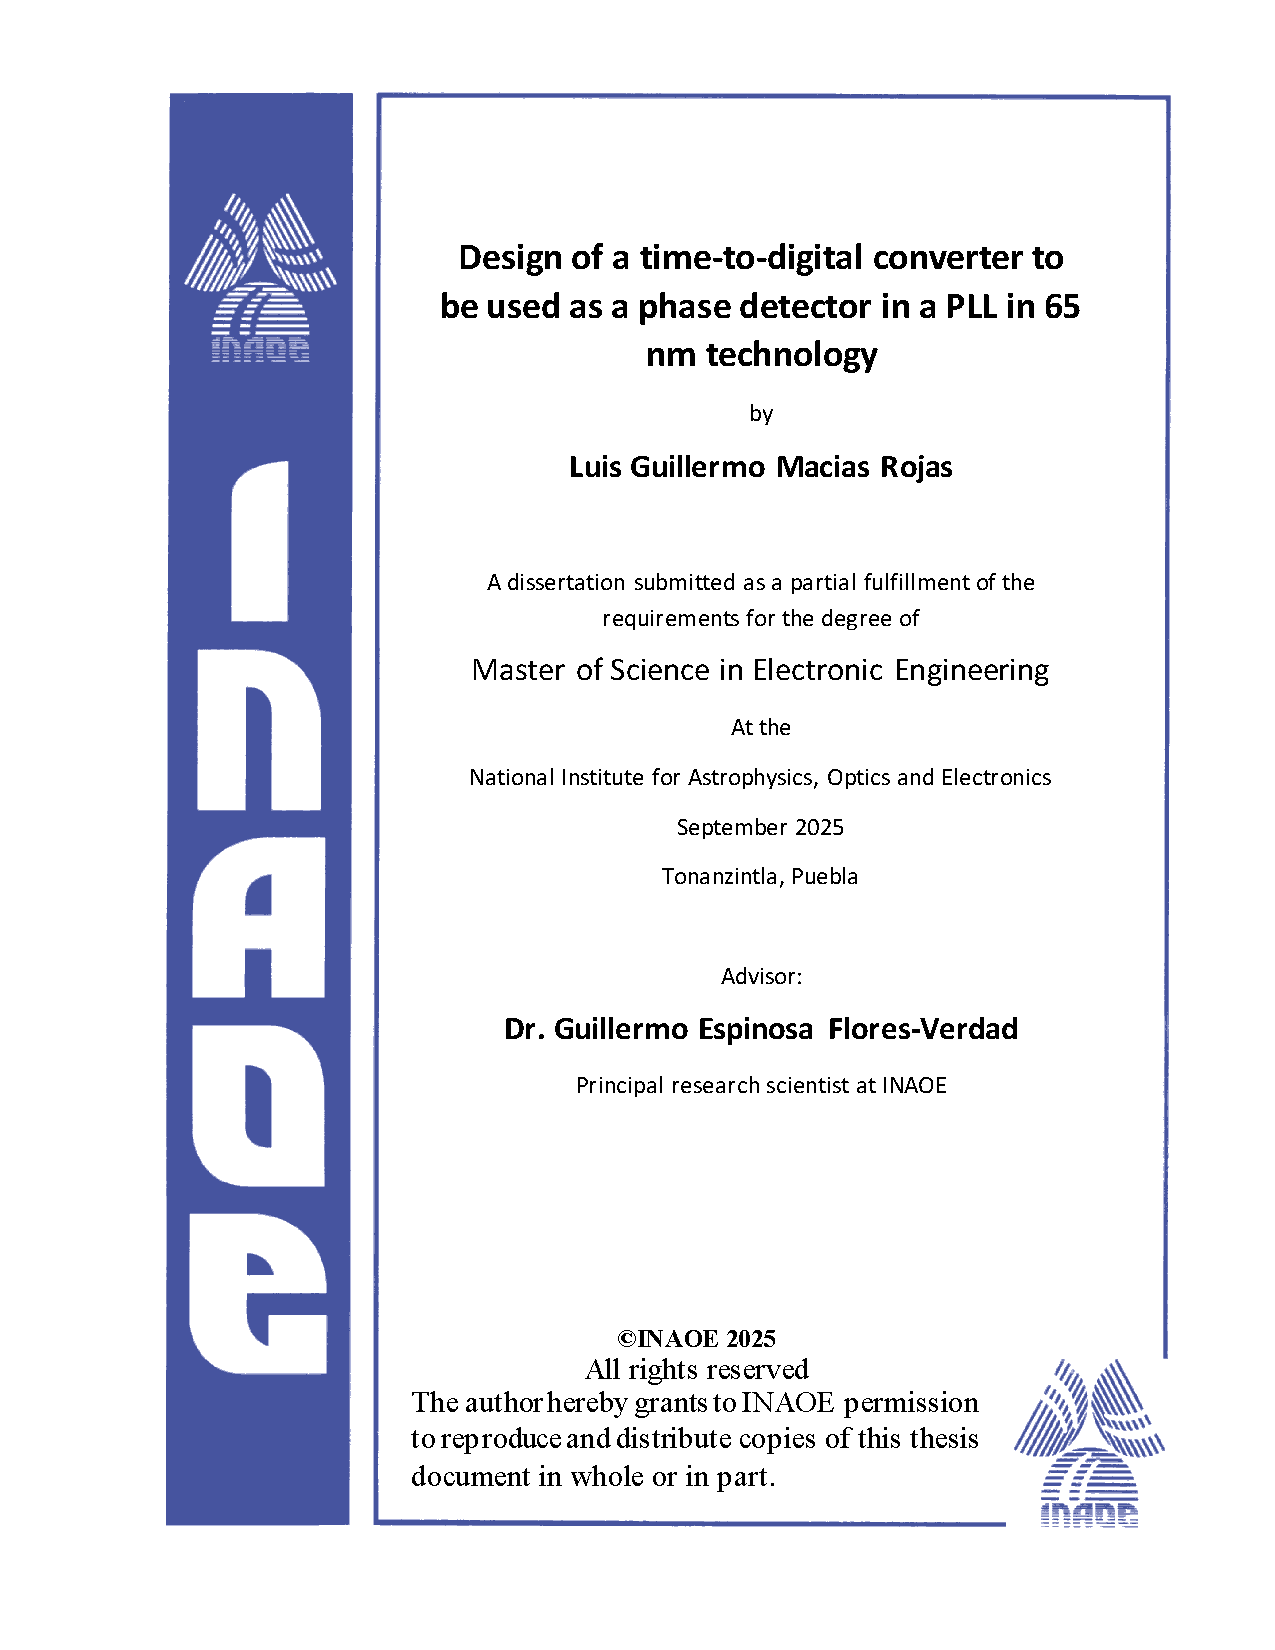
\includepdf{Portada_Tesis_Guillermo.pdf}    %Insert here PDF title page
    \end{titlepage}

    \fontfamily{phv}\selectfont % Selecting font family
    \chapter*{Abstract}
    The evolution of CMOS technology and the analog limitations that come with it move the direction of stable clock generation and frequency synthesis 
    towards all-digital phase-locked loops (ADPLL). At the heart of this type of systems is the time-to-digital converter (TDC), which directly replace the
    phase-frequency detector (PD) in analog PLLs. This revolution towards ADPLLs has sparked abundant innovation in the field of TDC design, yet there has
    been little focus in bipolar delay line TDCs.
    
    This thesis presents the analysis, design, and implementation of a 5-bit bipolar TDC that doubles the intrinsic dynamic range of standard architectures,
    alongside its corresponding digitally-controlled oscillator (DCO) based on a cross-coupled pair LC-tank.

    \chapter*{Acknowledgements}
    First and foremost, I would like to express my deepest gratitude to my supervisor, Dr. Guillermo Espinosa Flores-Verdad, for his invaluable guidance, unwavering support,
    and immense patience throughout this research. His expertise and insightful feedback were fundamental to the completion of this work.

    I am also grateful to M.S. Erick Arenas for his advice on the DCO design.
    \chapter*{Dedications}
    To my wife and parents, for their unconditional support and love.
    %%%%%%%%%%%%%%%%% Index $$$$$$$$$$$$$$$$$$$$$$$$
    \chapter*{}
    \tableofcontents
    \listoffigures
    \addcontentsline{toc}{chapter}{List of figures}
    \listoftables
    \addcontentsline{toc}{chapter}{List of tables}

    %\input{chapters/portada.tex}
    \chapter{Introduction}
\lipsum[1-2]
    \chapter{Theoretical framework}

\section{Phase-locked loop fundamentals}
\subsection{Basic structure}
\subsection{Key PLL parameters}
\subsubsection{Phase noise / jitter}
sggs
\subsubsection{Output frequency}
It is defined as the range of frequencies that the PLL is capable of generating and can be determined by the VCO output range and the division ratio of the feedback frequency divider. This
is a key metric in establishing the application of the PLL (e.g., clock generation or RF synthesizer) and it bears significant importance in the design process due to the tradeoff 
it has with the phase noise performance of the PLL.
\subsubsection{Loop bandwidth}
\subsubsection{Noise bandwidth}
dfbdfb
\subsubsection{Lock-in time}
dnsds
\subsubsection{Pull-in time}
danan
\subsubsection{Lock-in range}
adnna
\subsubsection{Pull-in range}
anan
\subsubsection{Pull-out range}
nana
\subsubsection{Hold range}
fdan
\subsubsection{SNR}
adfn
\subsubsection{Power consumption}
dfanna
\subsubsection{Spurious tones}
fdafdhdhdah

\subsection{Analog phase-locked loops}
dfanadn
\subsection{Linearized model}
daan
\subsection{Digital phase-locked loops}
anan
\section{Time-to-digital converters}
\subsection{Delay-locked loop fundamentals}
\subsection{TDC as a phase detector}

\section{65 nm CMOS technology}

    \chapter{Literature review}
\lipsum[1-2] \cite{van1994}
    \chapter{Methodology}
\lipsum[1-2]
    \chapter{Results}
\lipsum[1-2]
    \chapter{Discussion}
\lipsum[1-2]
    \chapter{Conclusion}
\lipsum[1-2]
    %%%%%%%%%%%%%%%%%%%%%%%%%%%%%%%%%%%%%%%%%%%%%%%%
    %\appendix
    %\chapter{Appendix}
\lipsum[4]

    \printbibliography  % Print bibliography
\end{document}